\documentclass{beamer}

\mode<presentation> {

%\usetheme{default}
%\usetheme{AnnArbor}
%\usetheme{Antibes}
%\usetheme{Bergen}
%\usetheme{Berkeley}
%\usetheme{Berlin}
%\usetheme{Boadilla}
%\usetheme{CambridgeUS}
%\usetheme{Copenhagen}
%\usetheme{Darmstadt}
%\usetheme{Dresden}
%\usetheme{Frankfurt}
%\usetheme{Goettingen}
%\usetheme{Hannover}
%\usetheme{Ilmenau}
%\usetheme{JuanLesPins}
%\usetheme{Luebeck}
\usetheme{Madrid}
%\usetheme{Malmoe}
%\usetheme{Marburg}
%\usetheme{Montpellier}
%\usetheme{PaloAlto}
%\usetheme{Pittsburgh}
%\usetheme{Rochester}
%\usetheme{Singapore}
%\usetheme{Szeged}
%\usetheme{Warsaw}


%\usecolortheme{albatross}
%\usecolortheme{beaver}
%\usecolortheme{beetle}
%\usecolortheme{crane}
%\usecolortheme{dolphin}
%\usecolortheme{dove}
%\usecolortheme{fly}
%\usecolortheme{lily}
%\usecolortheme{orchid}
%\usecolortheme{rose}
%\usecolortheme{seagull}
%\usecolortheme{seahorse}
%\usecolortheme{whale}
%\usecolortheme{wolverine}

%\setbeamertemplate{footline} % To remove the footer line in all slides uncomment this line
%\setbeamertemplate{footline}[page number] % To replace the footer line in all slides with a simple slide count uncomment this line

%\setbeamertemplate{navigation symbols}{} % To remove the navigation symbols from the bottom of all slides uncomment this line
}

\usepackage{graphicx} % Allows including images
\usepackage{booktabs} % Allows the use of \toprule, \midrule and \bottomrule in tables
\usepackage{amsfonts}
\usepackage{mathrsfs, bbold}
\usepackage{amsmath,amssymb,graphicx}
\usepackage{mathtools} % gather
\usepackage[export]{adjustbox} % right-aligned graphics

%----------------------------------------------------------------------------------------
%	TITLE PAGE
%----------------------------------------------------------------------------------------

\title["12"]{12: Computationally Efficient Markov chain Simulation}

% \author{Taylor} 
% \institute[UVA] 
% {
% University of Virginia \\
% \medskip
% \textit{} 
% }
% \date{} 

\begin{document}
%----------------------------------------------------------------------------------------

\begin{frame}
\titlepage 
\end{frame}

%----------------------------------------------------------------------------------------
\begin{frame}
\frametitle{Introduction}

We mention:
\begin{enumerate}
\item an example where adding auxiliary variables increases computational efficiency
\item a few tuning tips for Random-Walk Metropolis-Hastings
\item Metropolis-adjusted Langevin Algorithm (MALA)
\item Hamiltonian Monte Carlo (HMC)
\item Pseudo-Marginal Metropolis-Hastings (PMMH).
\end{enumerate}


\end{frame}


%----------------------------------------------------------------------------------------
\begin{frame}
\frametitle{Example: Data Augmentation}

\begin{itemize}
\item $y_1, \ldots, y_n \mid \mu, \sigma^2 \overset{\text{iid}}{\sim} t_{\nu}(\mu, \sigma^2)$
\item $\nu$ is assumed known
\item $p(y_i \mid \mu, \sigma^2) \propto \left(1 + \frac{1}{\nu}\left(\frac{y_i - \mu}{\sigma} \right)^2 \right)^{-(\nu+1)/2}$
\item $p(\mu) \propto 1$
\item $p(\sigma^2) \propto (\sigma^2)^{-1}$ (uniform for $\log \sigma$)
\end{itemize}
\pause

Normally we would do
$$
p(\mu, \sigma \mid y) \propto p(y \mid \mu, \sigma^2)p(\mu)p(\sigma^2)
$$
\newline

\end{frame}

%----------------------------------------------------------------------------------------
\begin{frame}[fragile]
\frametitle{Example: Data Augmentation}

Gibbs sampler not available :( 

\begin{center}
\includegraphics[width=100mm]{surf1}
\end{center}
see \verb|t_visualization.r|

\end{frame}


%----------------------------------------------------------------------------------------
\begin{frame}
\frametitle{Data Augmentation: auxiliary variables}

Instead, we introduce $V_i$ (hidden/latent/unobserved data):
\begin{itemize}
\item $p(y_i \mid V_i, \mu, \sigma^2) \sim N(\mu, V_i)$
\item $p(V_i \mid \sigma^2) \sim \mbox{Inv-}\chi^2(\nu,\sigma^2)$   
\item $\nu$ is assumed known still
\item $p(\mu) \propto 1$ still
\item $p(\sigma^2) \propto (\sigma^2)^{-1}$ (uniform for $\log \sigma$) still
\end{itemize}

% \begin{gather}
%   p(y_i \mid V_i, \mu, \sigma^2) \sim N(\mu, V_i)\\
%   %= (2\pi V_i)^{-1/2} \exp\left[- \frac{1}{2 V_i}\left(y_i - \mu \right)^2 \right] \\
%   p(V_i \mid \sigma^2) \sim \mbox{Inv-}\chi^2(\nu,\sigma^2)
%   %= \frac{(\nu/2)^{\nu/2}}{\Gamma(\nu/2) }\sigma^{\nu} V_i^{-(\nu/2 + 1)}\exp\left[- \nu \sigma^2/(2 V_i) \right]
% \end{gather}

\vspace{0.2cm}
$p(y_i \mid \mu, \sigma^2)$ is the same as before.
\end{frame}



%----------------------------------------------------------------------------------------
\begin{frame}
\frametitle{Data Augmentation: auxiliary variables}

We can show that
\begin{enumerate}
\item $V_i \mid \mu, \sigma^2, y \sim \text{Inv-}\chi^2\left(\nu + 1, \frac{ \nu \sigma^2 + (y_i - \mu)^2 }{\nu+1 } \right)$
\item $\mu \mid \sigma^2, V_{1:n}, y \sim \text{Normal}\left(\frac{\sum_i \frac{1}{V_i}y_i }{\sum_i \frac{1}{V_i} }, \frac{1}{ \sum_i \frac{1}{V_i} }\right)$ 
\item $\sigma^2 \mid \mu, V_{1:n}, y \sim \text{Gamma}\left(\frac{n \nu}{2}, \frac{\nu}{2}\sum_i \frac{1}{V_i} \right)$
\end{enumerate}

\end{frame}

%----------------------------------------------------------------------------------------
\begin{frame}[fragile]
\frametitle{Data Augmentation: auxiliary variables}

Note:
\begin{align*}
V_i \mid \mu, \sigma^2, y &\sim \text{Inv-}\chi^2\left(\nu + 1, \frac{ \nu \sigma^2 + (y_i - \mu)^2 }{\nu+1 } \right) \\
&= \text{Inv-Gamma}\left(\frac{\nu+1}{2}, \frac{ \nu \sigma^2 + (y_i - \mu)^2 }{2 }\right)
\end{align*}

\begin{center}
\includegraphics[width=40mm]{cond_dens_vi}
\end{center}
(see \verb|t_visualization.r|)
\newline

Near-zero values of $V_i$s lead to $\sigma^2$ being near zero, too.


\end{frame}
%----------------------------------------------------------------------------------------
\begin{frame}[fragile]
\frametitle{Data Augmentation: parameter expansion}

Add another parameter: $\alpha > 0$
\newline

Rename a few things:
\begin{gather}
\tau^2 = \sigma^2/\alpha^2 \\
U_i = V_i/\alpha^2 
\end{gather}

Assume a noninformative prior for $\alpha$: 
$$
p(\alpha^2) \propto (\alpha^2)^{-1}
$$

\end{frame}


%----------------------------------------------------------------------------------------
\begin{frame}
  \frametitle{Data Augmentation: parameter expansion}
\begin{itemize}
\item $p(y_i \mid V_i, \mu, \sigma^2) \sim N(\mu, \alpha^2 U_i)$
\item $p(U_i \mid \tau^2) \sim \mbox{Inv-}\chi^2(\nu,\tau^2)$   
\item $\nu$ is assumed known 
\item $p(\mu) \propto 1$ 
\item $p(\tau^2) \propto (\tau^2)^{-1}$ (uniform for $\log \tau$) 
\end{itemize}
Prove that the model is not identifiable in the full parameter space! However, the inference about $\mu$, $\alpha \tau$, and $\alpha^2U_i$ is still valid.
\end{frame}


%----------------------------------------------------------------------------------------
\begin{frame}
\frametitle{Data Augmentation: parameter expansion}

Posterior conditional distributions are similar:
\begin{enumerate}
\item $U_i \mid \alpha, \mu, \tau^2, y \sim \text{Inv-}\chi^2\left(\nu
    + 1, \frac{ \nu \tau^2 + ((y_i - \mu)/{\color{red} \alpha})^2 }{\nu+1 } \right)$
\item $\mu \mid {\color{red} \alpha}, \tau^2, U_{1:n}, y \sim \text{Normal}\left(\frac{\sum_i \frac{1}{{\color{red} \alpha}^2U_i}y_i }{\sum_i \frac{1}{{\color{red} \alpha}^2U_i} }, \frac{1}{ \sum_i \frac{1}{{\color{red} \alpha}^2U_i} }\right)$ 
\item $\tau^2 \mid \mu, U_{1:n}, y \sim \text{Gamma}\left(\frac{n
      \nu}{2}, \frac{\nu}{2}\sum_i \frac{1}{{\color{red} \alpha}^2U_i} \right)$
\item ${\color{red} \alpha} \mid \mu, \tau^2, U_{1:n}, y \sim \mbox{Inv-}\chi^2\left(n,
  \frac{1}{n}\sum_{i=1}^n \frac{(y_i - \mu_i)^2}{U_i}\right)$ 
\end{enumerate}

$\alpha$ breaks the dependence between $V_i = \alpha^2 U_i$ and $\tau^2$.
\end{frame}


%----------------------------------------------------------------------------------------
\begin{frame}
\frametitle{Random Walk M-H: Some Tricks}

Last chapter, when we were using the Metropolis-Hastings algorithm, we
need to specify the proposal's covariance matrix:

If $\theta$ is roughly normal,
$$
q(\theta^* \mid \theta^{t-1}) = \text{Normal}(\theta^{t-1}, \Sigma).
$$

The book recommends setting 
$$
\Sigma \approx \frac{2.4^2}{d} \operatorname{Var}(\theta \mid y).
$$
Here $d$ is the dimension of $\theta$. A rough approximation of the
posterior covariance matrix is required, e.g., Hession matrix at the
posterior mode.
\end{frame}


%----------------------------------------------------------------------------------------
\begin{frame}
  \frametitle{Random Walk M-H: Some Tricks}
Why set the proposal covariance matrix this way?
\vspace{0.2cm}

It is all about the efficiency of the posterior samples.
\vspace{0.2cm}

Specifically, our goal is to increase the {\bf rate} that a new independent $\theta$ being
generated. 
\vspace{0.2cm}

It can be shown that under the suggested proposal,
$q(\theta^* \mid \theta^{t-1}) = $ $\text{Normal}(\theta^{t-1},
\frac{2.4^2}{d} \operatorname{Var}(\theta \mid y))$, the efficiency is
$0.3/d$, meaning that, on average, every $d/0.3$ iterations a new independent
$\theta$ is drawn.
\vspace{0.2cm}

The efficiency is low when the dimension $d$ is large!!!
\end{frame}


%----------------------------------------------------------------------------------------
\begin{frame}
  \frametitle{Adaptive Metropolis-Hasting algorithm}
Adaptive MH is aimed to improve the acceptance rate:

Initial stage:
\begin{itemize}
\item Start simulations with a fixed MH algorithm using proposals like $q(\theta^* \mid \theta^{t-1}) = $ $\text{Normal}(\theta^{t-1},
\frac{2.4^2}{d} \operatorname{Var}(\theta \mid y))$ 
\end{itemize}
Adaptive stage:
\begin{itemize}
\item Update the jumping rule as $q(\theta^* \mid \theta^{t-1}) = \text{Normal}(\theta^{t-1},
\Sigma)$, where $\Sigma$ is estimated from the simulation in initial
stage.
\item (Optional, needs parallel simulations) Adjust the scale of the
  jumping distribution until an acceptance rate of 0.44 in one
  dimension or 0.23 when parameters are updated as a vector.
\end{itemize}

Note: if $\Sigma$ is the same as the target distribution, the jumping
rule, $q(\theta^* \mid \theta^{t-1}) = $ $\text{Normal}(\theta^{t-1},
\frac{2.4^2}{d} \Sigma)$, has acceptance rate 0.44 in one
  dimension or 0.23 when parameters are updated as a vector.
\end{frame}


%----------------------------------------------------------------------------------------
\begin{frame}
  \frametitle{Slice sampling}
To sample from a distribution, simply sample uniformly from the
region under the density function and consider only the horizontal
coordinates.
\begin{center}
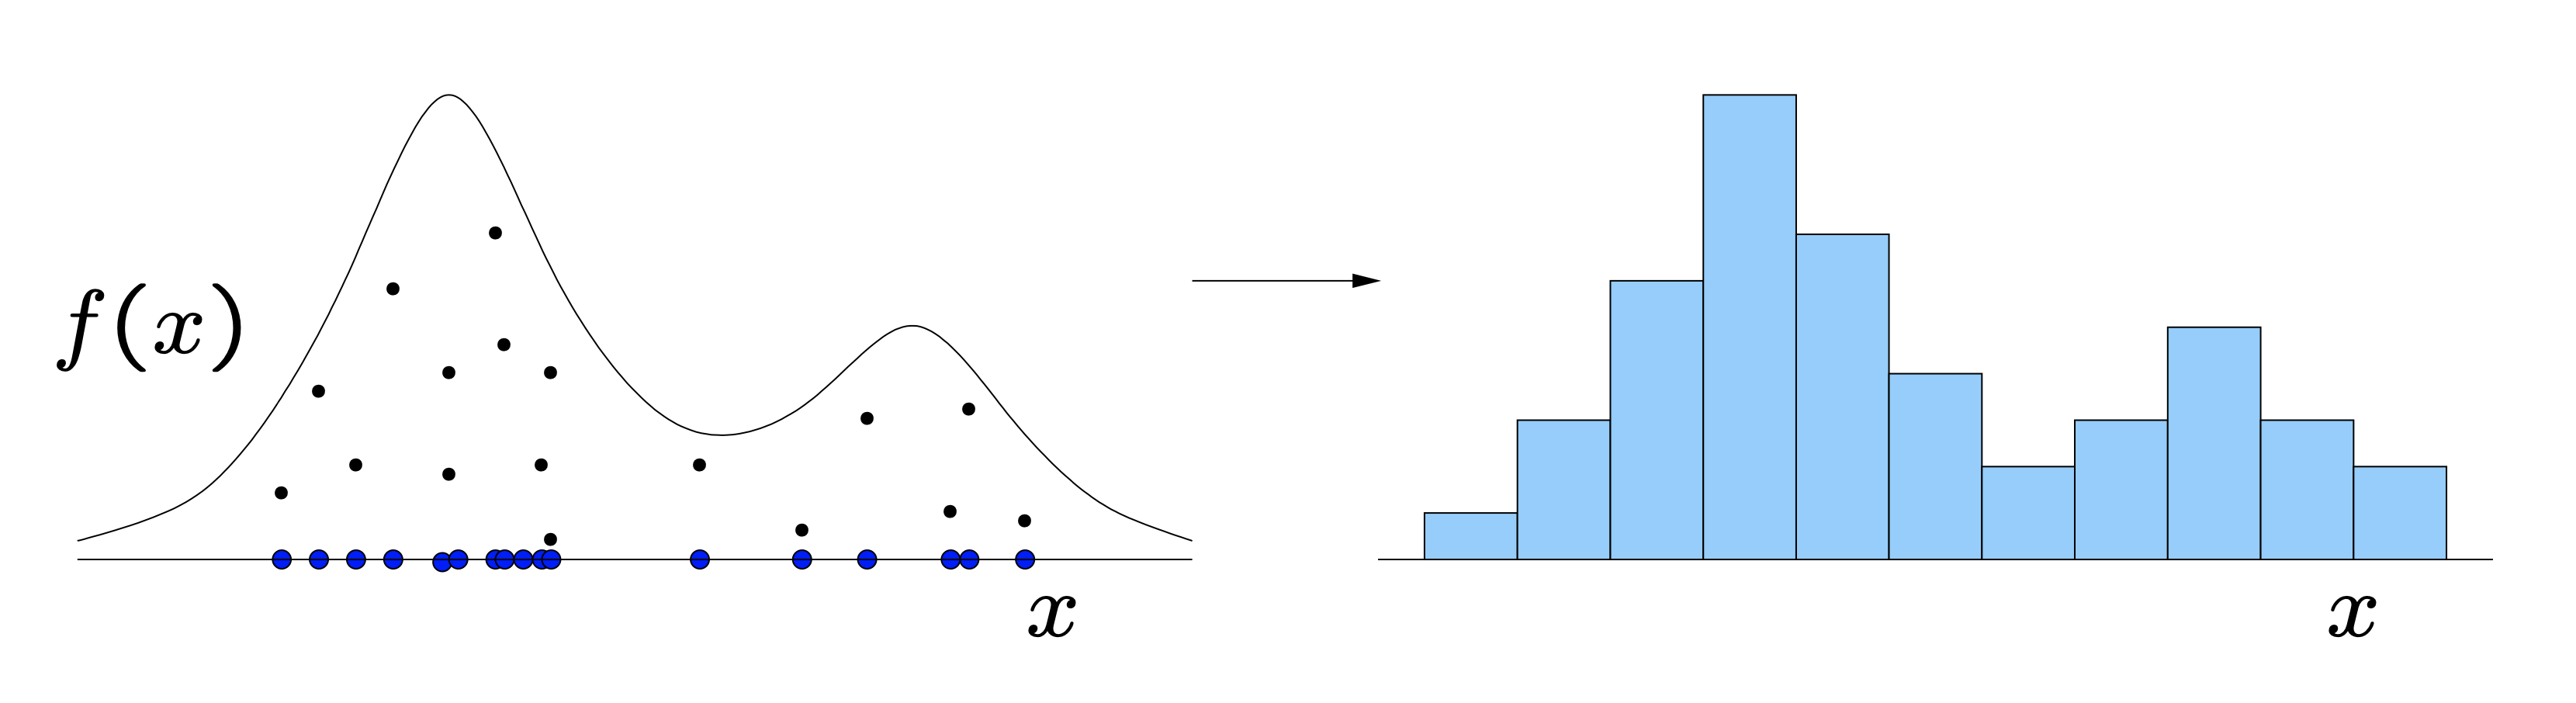
\includegraphics[width=120mm]{slice_sampling}
\end{center}
\end{frame}



%----------------------------------------------------------------------------------------
\begin{frame}
  \frametitle{Slice sampling}
One way to do this is
\begin{itemize}
\item Introduce latent (auxiliary) variables
\item Use Gibbs sampling on the area beneath the density
\end{itemize}
\vspace{0.2cm}

Suppose we wish to sample from $f(x)$, it is equivalent to:
\begin{itemize}
\item $y \mid x \sim \mbox{Uniform}(0, f(x))$, then $f(x,y)$ is
  constant over $\{(x,y): 0 \leq y \leq f(x)\}$.
\item $x \mid y \propto f(x,y) \sim \mbox{Uniform}(S(y))$, where $S(y)
  = \{x: y \leq f(x)\}$  
\end{itemize}
\end{frame}


%----------------------------------------------------------------------------------------
\begin{frame}
  \frametitle{Slice sampling}
  This leads to an iterative algorithm:
  \begin{itemize}
  \item $y_i \mid x_{i-1} \sim \mbox{Uniform}(0, f(x_{i-1}))$
  \item $x_i \mid y_i \sim \mbox{Uniform}(S(y_i))$
  \end{itemize}
\vspace{0.2cm}

No need to specify proposal distributions as needed by MH or rejection sampling. 
\vspace{0.2cm}

Determining the slice $S(y)$ can be tricky!
\end{frame}


%----------------------------------------------------------------------------------------
\begin{frame}
  \frametitle{Slice sampling: example for normal distribution}
Suppose $x \sim \mbox{Normal}(0,1)$, so $f(x) \propto g(x) =
\exp(-x^2/2)$,

then the slice through the density is 
\[
S(y) = \{x: -\sqrt{-2\log(y)} \leq x \leq \sqrt{-2\log(y)}\}.
\]  

First five iterations of the slice sampler for the standard normal
example:
\begin{center}
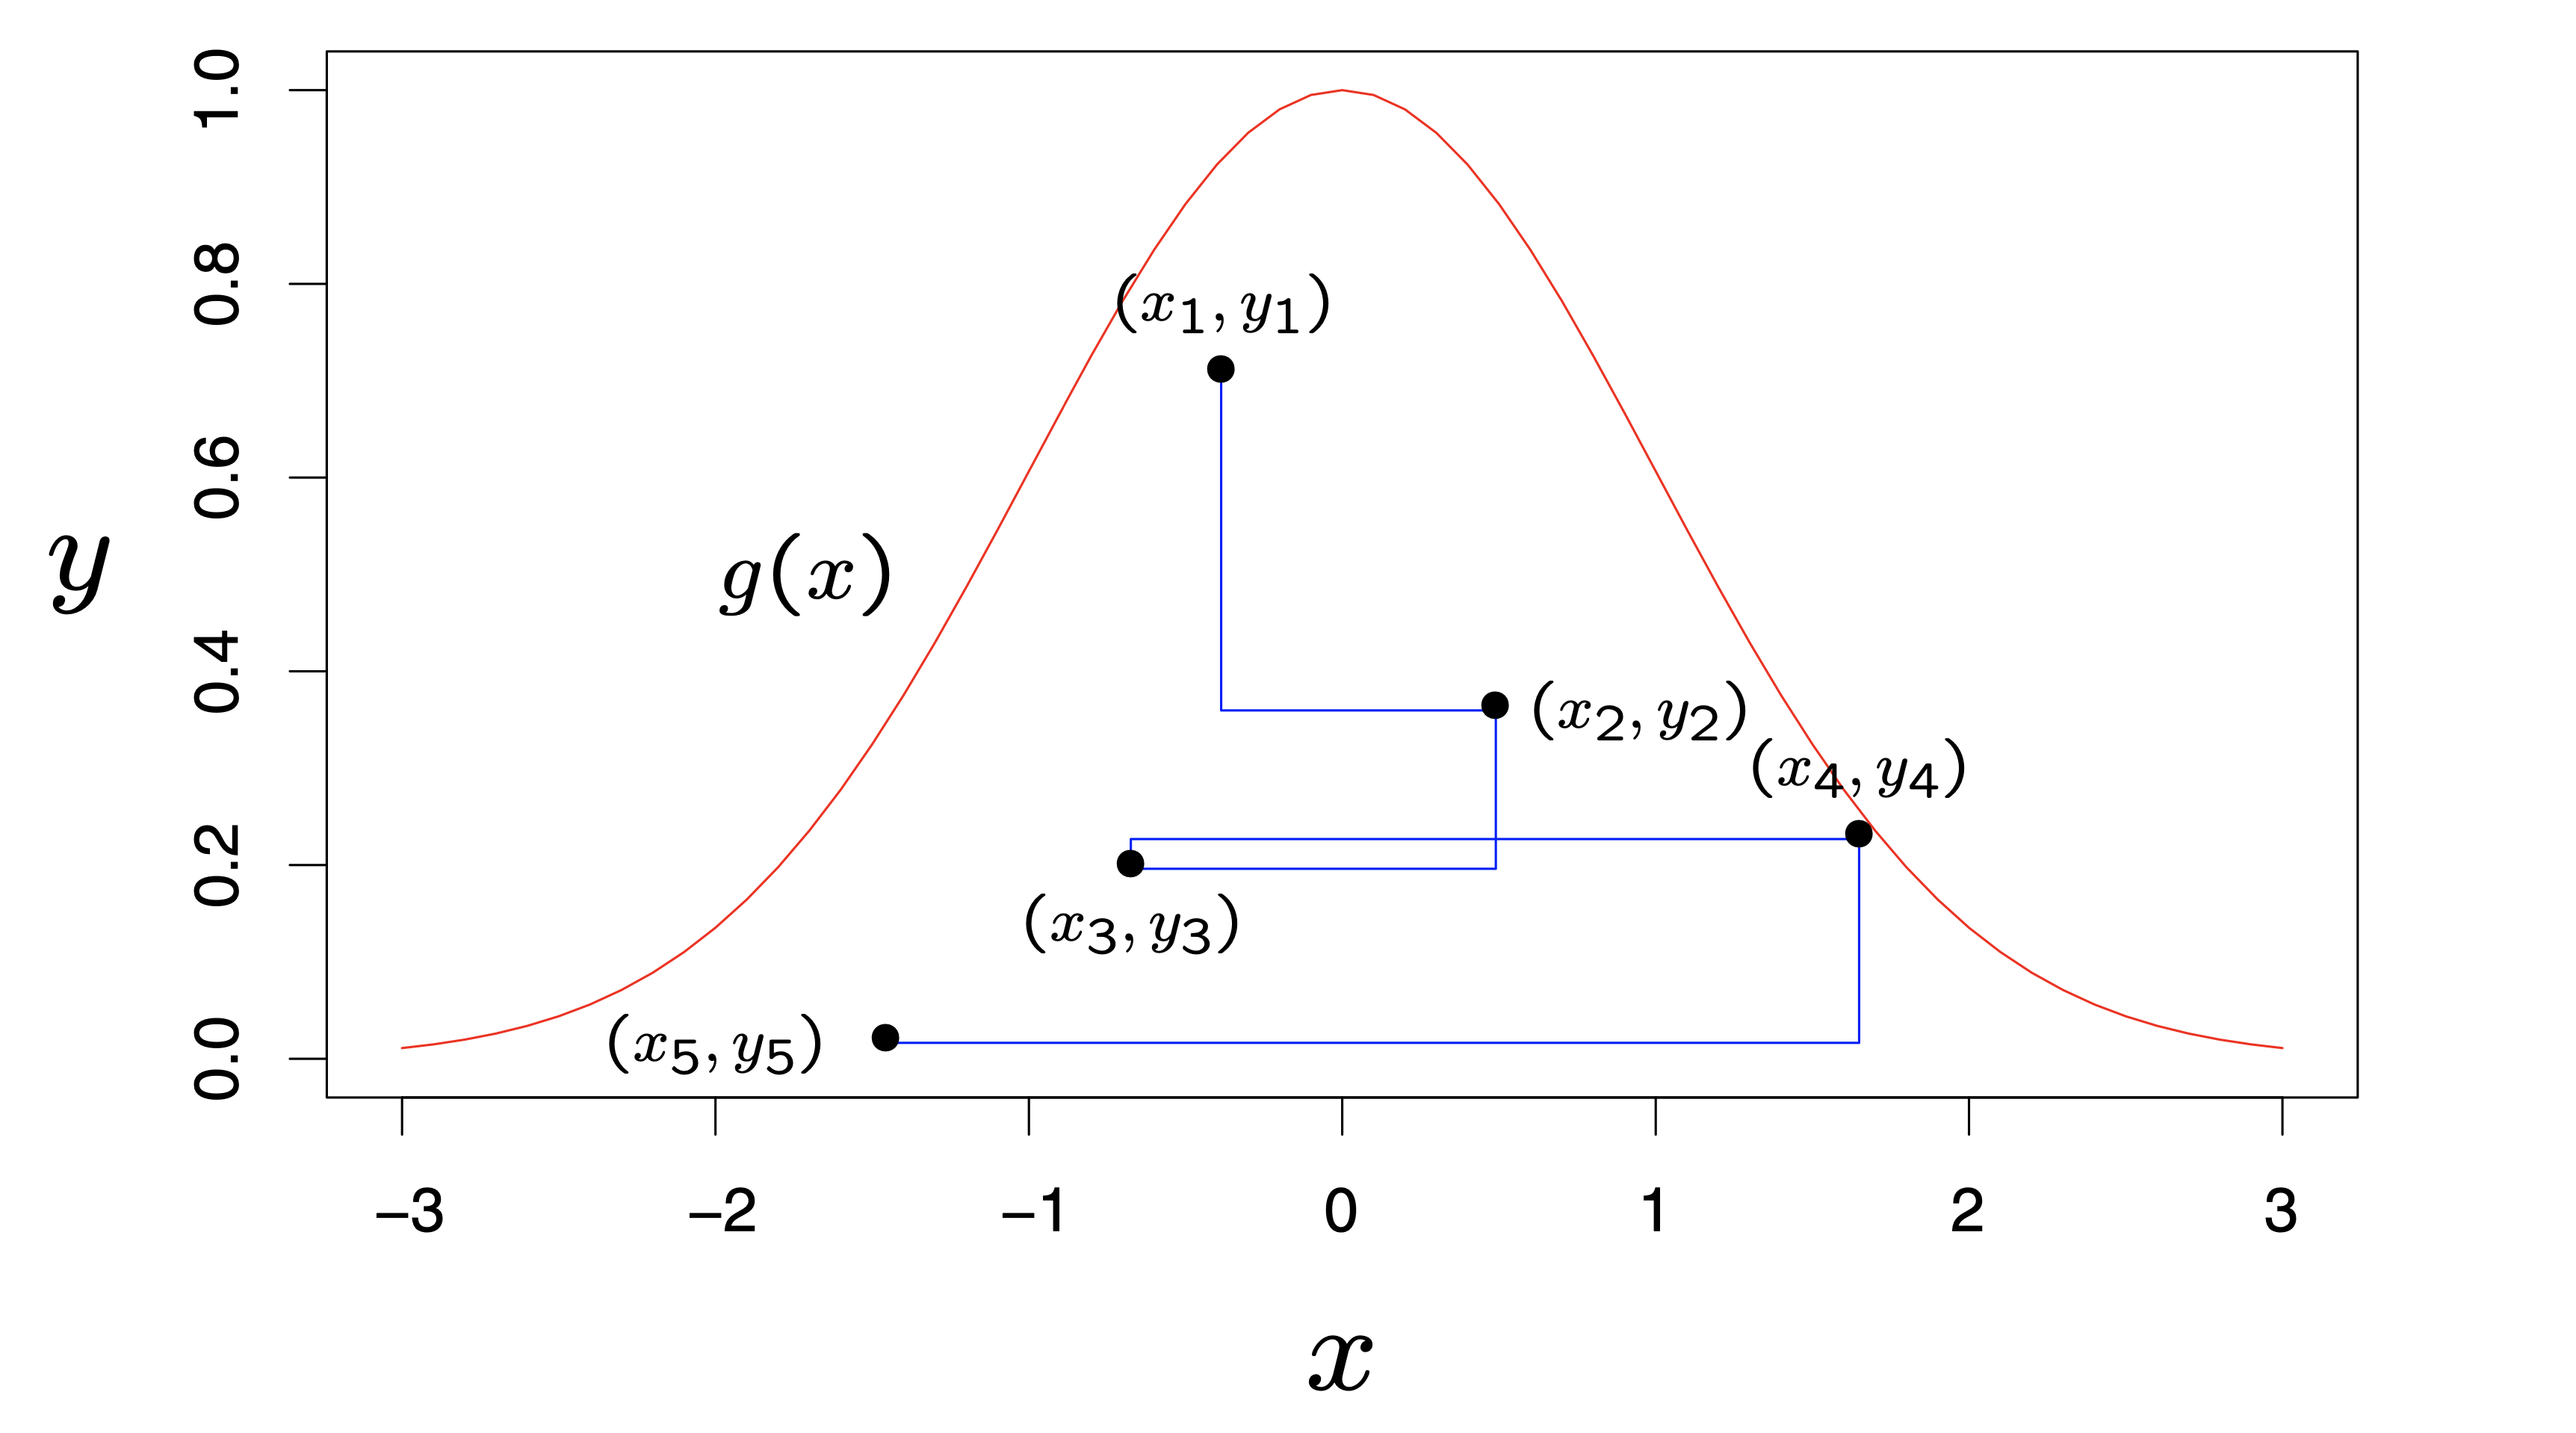
\includegraphics[width=120mm, height=55mm]{slice_sampling_normal}
\end{center}
\end{frame}


%----------------------------------------------------------------------------------------
\begin{frame}
  \frametitle{Sampling from multi-modal distribution: simulated tempering}
Let $p(\theta)$ be the target (unnormalized) density. Consider 
\[
q_k(\theta) \propto p(\theta)^{1/T_k}
\]
for a set of ``temperature" parameters $T_k > 0$, $k = 0, 1, \ldots,
K$, where $T_0 = 1$ and $q_0(\theta) = p(\theta)$.
\vspace{0.2cm}

For $T_k$ large (high temperature), the density $q_k$ will be more
flat than $q_0$.   

Simulated tempering constructs a Markov chain with augmented state $(\theta^t,
s^t)$ at time $t$ with $s^t$ an integer indicating the current temperature.
\end{frame}


%----------------------------------------------------------------------------------------
\begin{frame}
  \frametitle{Sampling from multi-modal distribution: simulated
    tempering}
The algorithm is an Metropolis-Hasting algorithm leading to a composite Markov
chain:
\begin{itemize}
\item Propose a new state for $\theta^t$: $\theta^{t}$ is then generated using Markov chain simulation
corresponding to stationary distribution $q_{s^{t-1}}$.
\item An MH step for $s^{t}$: \\
 proposing $s^t$ according to $P(s^t = k) \propto J_{s^{t-1}, k}$\\
 accept with probability $\min(r, 1)$, where 
\[
r = \frac{c_k q_k(\theta^{t}) J_{k s^{t-1}}}{c_{s^{t-1}} q_{s^{t-1}}(\theta^{t}) J_{s^{t-1} k}}
\]
$c_k$ is the normalizing constant for $q_k$.
\end{itemize}
Once the composite Markov chain is simulated for $t = 1, \ldots, T$,
only $\theta^t$ corresponding to $s^t = 0$ are kept for inference
about $q_0$.
\end{frame}

%%% Local Variables:
%%% mode: latex
%%% TeX-master: t
%%% End:
\end{document}